%%%%%%%%%%%%%%%%%%%%%%%%%%%%%%%%%%%%%%%%%%%%%%%%%%%%%%%%%%%%%%%%%%%%%%
%%  Copyright by Wenliang Du.                                       %%
%%  This work is licensed under the Creative Commons                %%
%%  Attribution-NonCommercial-ShareAlike 4.0 International License. %%
%%  To view a copy of this license, visit                           %%
%%  http://creativecommons.org/licenses/by-nc-sa/4.0/.              %%
%%%%%%%%%%%%%%%%%%%%%%%%%%%%%%%%%%%%%%%%%%%%%%%%%%%%%%%%%%%%%%%%%%%%%%

\newcommand{\commonfolder}{../../common-files}

\documentclass[11pt]{article}

\usepackage[most]{tcolorbox}
\usepackage{times}
\usepackage{epsf}
\usepackage{epsfig}
\usepackage{amsmath, alltt, amssymb, xspace}
\usepackage{wrapfig}
\usepackage{fancyhdr}
\usepackage{url}
\usepackage{verbatim}
\usepackage{fancyvrb}
\usepackage{adjustbox}
\usepackage{listings}
\usepackage{color}
\usepackage{subfigure}
\usepackage{cite}
\usepackage{sidecap}
\usepackage{pifont}
\usepackage{mdframed}
\usepackage{textcomp}
\usepackage{enumitem}
\usepackage{hyperref}


% Horizontal alignment
\topmargin      -0.50in  % distance to headers
\oddsidemargin  0.0in
\evensidemargin 0.0in
\textwidth      6.5in
\textheight     8.9in 

\newcommand{\todo}[1]{
\vspace{0.1in}
\fbox{\parbox{6in}{TODO: #1}}
\vspace{0.1in}
}


\newcommand{\unix}{{\tt Unix}\xspace}
\newcommand{\linux}{{\tt Linux}\xspace}
\newcommand{\minix}{{\tt Minix}\xspace}
\newcommand{\ubuntu}{{\tt Ubuntu}\xspace}
\newcommand{\setuid}{{\tt Set-UID}\xspace}
\newcommand{\openssl} {\texttt{openssl}}

% Arrows
\newcommand{\pointleft}[1]{\reflectbox{\ding{217}} \textbf{\texttt{#1}}}
\newcommand{\pointright}[1]{\ding{217} \textbf{\texttt{#1}}}
\newcommand{\pointupleft}[1]{\reflectbox{\ding{218}} \textbf{\texttt{#1}}}

% Line numbers
\newcommand{\lineone}{\ding{192}\xspace}
\newcommand{\linetwo}{\ding{193}\xspace}
\newcommand{\linethree}{\ding{194}\xspace}
\newcommand{\linefour}{\ding{195}\xspace}
\newcommand{\linefive}{\ding{196}\xspace}
\newcommand{\linesix}{\ding{197}\xspace}
\newcommand{\lineseven}{\ding{198}\xspace}
\newcommand{\lineeight}{\ding{199}\xspace}
\newcommand{\linenine}{\ding{200}\xspace}


% Fancy headers
\pagestyle{fancy}
\lhead{\bfseries SEED Labs}
\chead{}
\rhead{\small \thepage}
\lfoot{}
\cfoot{}
\rfoot{}


\definecolor{dkgreen}{rgb}{0,0.6,0}
\definecolor{gray}{rgb}{0.5,0.5,0.5}
\definecolor{mauve}{rgb}{0.58,0,0.82}
\definecolor{lightgray}{gray}{0.90}


\lstset{%
  frame=none,
  language=,
  backgroundcolor=\color{lightgray},
  aboveskip=3mm,
  belowskip=3mm,
  showstringspaces=false,
%  columns=flexible,
  basicstyle={\small\ttfamily},
  numbers=none,
  numberstyle=\tiny\color{gray},
  keywordstyle=\color{blue},
  commentstyle=\color{dkgreen},
  stringstyle=\color{mauve},
  breaklines=true,
  breakatwhitespace=true,
  tabsize=3,
  columns=fullflexible,
  keepspaces=true,
  escapeinside={(*@}{@*)}
}

\newcommand{\newnote}[1]{
\vspace{0.1in}
\noindent
\fbox{\parbox{1.0\textwidth}{\textbf{Note:} #1}}
%\vspace{0.1in}
}


%% Submission
\newcommand{\seedsubmission}{You need to submit a detailed lab report, with screenshots,
to describe what you have done and what you have observed.
You also need to provide explanation
to the observations that are interesting or surprising.
Please also list the important code snippets followed by
explanation. Simply attaching code without any explanation will not
receive credits.}

%% Book
\newcommand{\seedbook}{\textit{Computer \& Internet Security: A Hands-on Approach}, 3rd
Edition, by Wenliang Du. See details at \url{https://www.handsonsecurity.net}.\xspace}

\newcommand{\seedisbook}{\textit{Internet Security: A Hands-on Approach}, 3rd
Edition, by Wenliang Du. See details at \url{https://www.handsonsecurity.net}.\xspace}

\newcommand{\seedcsbook}{\textit{Computer Security: A Hands-on Approach}, 3rd
Edition, by Wenliang Du. See details at \url{https://www.handsonsecurity.net}.\xspace}

\newcommand{\seedcibook}{\textit{Computer \& Internet Security: A Hands-on Approach}, 3rd
Edition, by Wenliang Du. See details at \url{https://www.handsonsecurity.net}.\xspace}

%% Videos
\newcommand{\seedisvideo}{\textit{Internet Security: A Hands-on Approach},
by Wenliang Du. See details at \url{https://www.handsonsecurity.net/video.html}.\xspace}

\newcommand{\seedcsvideo}{\textit{Computer Security: A Hands-on Approach},
by Wenliang Du. See details at \url{https://www.handsonsecurity.net/video.html}.\xspace}

%% Lab Environment
\newcommand{\seedenvironment}{This lab has been tested on our pre-built
Ubuntu 16.04 VM, which can be downloaded from the SEED website.\xspace}

\newcommand{\seedenvironmentA}{This lab has been tested on our pre-built
Ubuntu 16.04 VM, which can be downloaded from the SEED website.\xspace}

\newcommand{\seedenvironmentB}{This lab has been tested on our pre-built
Ubuntu 20.04 VM, which can be downloaded from the SEED website.\xspace}

\newcommand{\seedenvironmentC}{This lab has been tested on the SEED
Ubuntu 20.04 VM. You can download a pre-built image from the SEED website, 
and run the SEED VM on your own computer. However,
most of the SEED labs can be conducted on the cloud, and 
you can follow our instruction to create a SEED VM on the cloud.\xspace}

\newcommand{\seedenvironmentAB}{This lab has been tested on our pre-built
Ubuntu 16.04 and 20.04 VMs, which can be downloaded from the SEED website.\xspace}

\newcommand{\nodependency}{Since we use containers to set up the lab environment, 
this lab does not depend much on the SEED VM. You can do this lab
using other VMs, physical machines, or VMs on the cloud.\xspace}

\newcommand{\adddns}{You do need to add the required IP address mapping to
the \texttt{/etc/hosts} file.\xspace}






\newcommand{\seedlabcopyright}[1]{
\vspace{0.1in}
\fbox{\parbox{6in}{\small Copyright \copyright\ {#1}\ \ by Wenliang Du.\\
      This work is licensed under a Creative Commons
      Attribution-NonCommercial-ShareAlike 4.0 International License.
      If you remix, transform, or build upon the material, 
      this copyright notice must be left intact, or reproduced in a way that is reasonable to
      the medium in which the work is being re-published.}}
\vspace{0.1in}
}






\lhead{\bfseries SEED Labs -- ARP Cache Poisoning Attack Lab}
\newcommand{\arpFigs}{./Figs}


\begin{document}



\begin{center}
{\LARGE ARP Cache Poisoning Attack Lab}
\end{center}

\seedlabcopyright{2019}



% *******************************************
% SECTION
% ******************************************* 
\section{Overview}


The Address Resolution Protocol (ARP) is a communication protocol used for discovering the link
layer address, such as the MAC address, given an IP address. The ARP protocol is a very simple
protocol, and it does not implement any security measure. 
The ARP cache poisoning attack is a common attack against the ARP protocol. 
Using such an attack, attackers can fool the victim into accepting
forged IP-to-MAC mappings. This can cause the victim's packets to be 
redirected to the computer with the forged MAC address, leading to
potential man-in-the-middle attacks.


The objective of this lab is for students to gain the first-hand experience on the ARP cache
poisoning attack, and learn what damages can be caused by such an attack.
In particular, students will use the ARP attack to launch a man-in-the-middle attack,  
where the attacker can intercept and modify the packets between the two victims A and B. 
Another objective of this lab is for students to practice 
packet sniffing and spoofing skills, as these are 
essential skills in network security, and they are the building blocks
for many network attack and defense tools. 
Students will use Scapy to conduct lab tasks. 
This lab covers the following topics:


\begin{itemize}[noitemsep]
\item The ARP protocol
\item The ARP cache poisoning attack
\item Man-in-the-middle attack
\item Scapy programming
\end{itemize}
 


\paragraph{Videos.}
Detailed coverage of the ARP protocol and attacks can be found in the following:

\begin{itemize}
\item Section 3 of the SEED Lecture at Udemy, \seedisvideo
\end{itemize}


\paragraph{Lab environment.} \seedenvironmentC




% *******************************************
% SECTION
% *******************************************
\section{Environment Setup using Container}

In this lab, we need three machines. We use 
containers to set up the lab environment, which is depicted 
in Figure~\ref{arp:fig:labsetup}.
In this setup, we have an attacker machine (Host M),
which is used to launch attacks against the other two machines, Host A and
Host B.  These three machines must be on the same LAN,
because the ARP cache poisoning attack is limited to LAN. We use 
containers to set up the lab environment.

\begin{figure}[htb]
\begin{center}
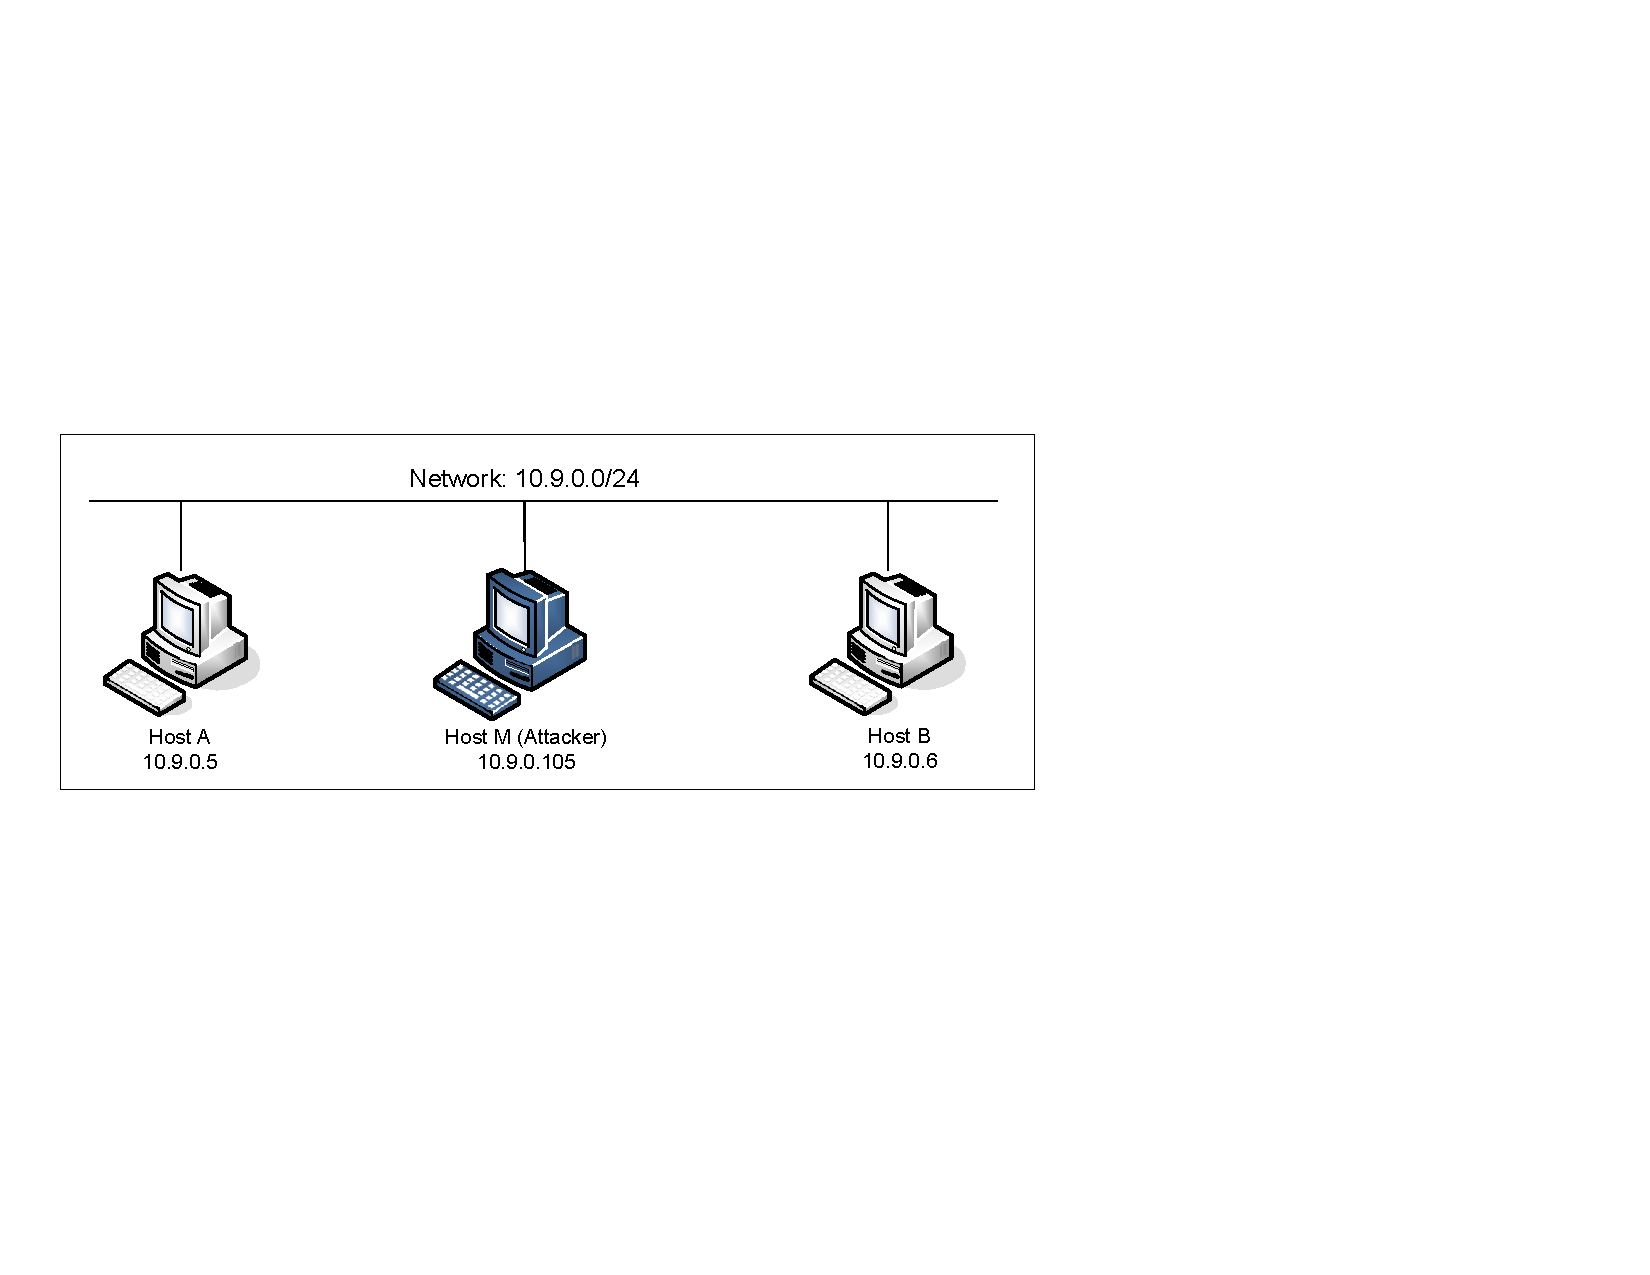
\includegraphics[width=0.8\textwidth]{\commonfolder/Figs/ARP_onelan.pdf}
\end{center}
\caption{Lab environment setup}
\label{arp:fig:labsetup}
\end{figure}
 

% -------------------------------------------
% SUBSECTION
% -------------------------------------------
\subsection{Container Setup and Commands}

%%%%%%%%%%%%%%%%%%%%%%%%%%%%%%%%%%%%%%%%%%%%
We provide a pre-built emulator in two different forms: Python code
and container files. The container files are generated from
the Python code, but students need to install the SEED Emulator source
code from the GitHub to run the Python code. The container files
can be directly used without the emulator source code.
Instructors who would like to customize the emulator can modify the Python
code, generate their own container files, and then provide the
files to students, replacing the ones included in the
lab setup file. See the \texttt{README.md} file for instructions. 


\paragraph{Download the emulator files.}
Please download the \texttt{Labsetup.zip} file from the web page, and
unzip it. The files inside the container folder are the actual 
emulation files (container files); they are generated by the Python code.
The name of the container folder is called \texttt{output/} for most labs,
but if a lab has multiple emulators, it will use 
different folder names. The actual names will be given in the lab task.


\paragraph{Start the emulation.}
We will directly use the files in the container folder.
Go to this folder, and run the docker commands
to build and start the containers. We recommend that you run the emulator inside
the provided SEED Ubuntu 20.04 VM, but doing it in a generic Ubuntu 20.04 operating system
should not have any problem, as long as the docker software is installed.
Readers can find the docker manual from
\href{https://github.com/seed-labs/seed-labs/blob/master/manuals/docker/SEEDManual-Container.md}
{\underline{this link}}.
If this is the first time you set up a SEED lab environment
using containers, it is very important that you read 
the user manual. 


In the following, we list some of the commonly
used commands related to Docker and Compose. 
Since we are going to use 
these commands very frequently, we have created aliases for them
in the \texttt{.bashrc} file (in our provided SEEDUbuntu 20.04 VM).

\begin{lstlisting}
$ docker-compose build  # Build the container images
$ docker-compose up     # Start the containers
$ docker-compose down   # Shut don the containers


// Aliases for the Compose commands above
$ dcbuild       # Alias for: docker-compose build
$ dcup          # Alias for: docker-compose up
$ dcdown        # Alias for: docker-compose down
\end{lstlisting}


All the containers will be running in the background. To run
commands on a container, we often need to get a shell on
that container. We first need to use the \texttt{"docker ps"}  
command to find out the ID of the container, and then
use \texttt{"docker exec"} to start a shell on that 
container. We have created aliases for them in
the \texttt{.bashrc} file.

\begin{lstlisting}
$ dockps        // Alias for: docker ps --format "{{.ID}}  {{.Names}}" 
$ docksh <id>   // Alias for: docker exec -it <id> /bin/bash

// The following example shows how to get a shell inside hostC
$ dockps
b1004832e275  hostA-10.9.0.5
0af4ea7a3e2e  hostB-10.9.0.6
9652715c8e0a  hostC-10.9.0.7

$ docksh 96
root@9652715c8e0a:/#  

// Note: If a docker command requires a container ID, you do not need to 
//       type the entire ID string. Typing the first few characters will 
//       be sufficient, as long as they are unique among all the containers. 
\end{lstlisting}


If you encounter problems when setting up the lab environment, 
please read the ``Common Problems'' section of the manual
for potential solutions.



\paragraph{Set the terminal title.} 
We may need to get into several containers using the terminal.
We will likely create several terminal tabs, and switch back
and forth among these tabs. We can easily get lost, because
it is difficult to know which tab runs which container. 
To solve this problem, once we
are inside a container, we can set the terminal title using
one of the following commands (it sets the title to \texttt{"New Title"}).

\begin{lstlisting}
# set_title New Title
# st New Title       (*@\pointleft{st} is an alias of set\_title@*)
\end{lstlisting}



%%%%%%%%%%%%%%%%%%%%%%%%%%%%%%%%%%%%%%%%%%%%


% -------------------------------------------
% SUBSECTION
% -------------------------------------------
\subsection{About the Attacker Container}

In this lab, we can either use the VM or the attacker container
as the attacker machine. If you look at the Docker Compose file, you will
see that the attacker container is configured differently from the other
containers. Here are the differences:

\begin{itemize}
\item \textit{Shared folder.} When we use the attacker container
to launch attacks, we need to put the attacking code inside
the container.
%%%%%%%%%%%%%%%%%%%%%%%%%%%%%%%%%%%%%%%%%%%%%%%
Code editing is more convenient inside the VM than in containers, 
because we can use our favorite editors.
In order for the VM and container to share files, 
we have created a shared folder between the VM and the container
using the Docker \texttt{volumes}.
If you look at the Docker Compose file, you will find out that
we have added the following entry to some of the containers.
It indicates mounting the \texttt{./volumes} folder on the host
machine (i.e., the VM) to the \texttt{/volumes} folder inside the container.
We will write our code in the \texttt{./volumes} folder (on the VM), so they
can be used inside the containers.

\begin{lstlisting}
volumes:
       - ./volumes:/volumes
\end{lstlisting}


%%%%%%%%%%%%%%%%%%%%%%%%%%%%%%%%%%%%%%%%%%%%%%%

\item \textit{Privileged mode.}
%%%%%%%%%%%%%%%%%%%%%%%%%%%%%%%%%%%%%%%%%%%%%%%
To be able to modify kernel parameters at runtime (using \texttt{sysctl}),
such as enabling IP forwarding, a container needs to be privileged.
This is achieved by including the following entry
in the Docker Compose file for the container.

\begin{lstlisting}
privileged: true
\end{lstlisting}


%%%%%%%%%%%%%%%%%%%%%%%%%%%%%%%%%%%%%%%%%%%%%%%

\end{itemize}


% -------------------------------------------
% SUBSECTION
% -------------------------------------------
\subsection{Packet Sniffing} 

%%%%%%%%%%%%%%%%%%%%%%%%%%%%%%%%%%%%%%%%%%%%%%%

Being able to sniff packets is very
important in this lab, because if things do not go as expected, being
able to look at where packets go can help us identify the problems.
There are several different ways to do packet sniffing:


\begin{itemize}
\item Running \texttt{tcpdump} on containers.
We have already installed \texttt{tcpdump}
on each container. To sniff the packets going through a particular
interface, we just need to find out the interface name, and then do the
following (assume that the interface name is \texttt{eth0}):

\begin{lstlisting}
# tcpdump -i eth0 -n
\end{lstlisting}

It should be noted that inside containers, due to the isolation created by
Docker, when we run \texttt{tcpdump} inside a container,
we can only sniff the packets going in and out of this container.
We won't be able to sniff the packets between other containers. 
However, if a container uses the \texttt{host} mode in its 
network setup, it can sniff other containers' packets. 


\item Running \texttt{tcpdump} on the VM. If we run \texttt{tcpdump}
on the VM, we do not have the restriction on the containers, and
we can sniff all the packets going among containers. The interface
name for a network is different on the VM than on the container.
On containers, each interface name usually starts with \texttt{eth};
on the VM, the interface name for the network created
by Docker starts with \texttt{br-}, followed by the ID of the network.
You can always use the \texttt{ip address} command to get the
interface name on the VM and containers.

\item We can also run Wireshark on the VM to sniff packets.
Similar to \texttt{tcpdump}, we need to select what interface
we want Wireshark to sniff on.
\end{itemize}


%%%%%%%%%%%%%%%%%%%%%%%%%%%%%%%%%%%%%%%%%%%%%%%



% *******************************************
% SECTION
% ******************************************* 
\section{Task 1: ARP Cache Poisoning}


The objective of this task is to use packet spoofing to launch an ARP cache poisoning attack on
a target, such that when two victim machines A and B try to communicate with each other, their
packets will be intercepted by the attacker, who can make changes to the packets, and can thus
become the man in the middle between A and B. This is called Man-In-The-Middle (MITM) attack.
In this task, we focus on the ARP cache poisoning part.
The following code skeleton shows how to construct an ARP packet using Scapy. 

\begin{lstlisting}
#!/usr/bin/env python3
from scapy.all import *

E = Ether()
A = ARP()
A.op = 1     # 1 for ARP request; 2 for ARP reply

pkt = E/A
sendp(pkt)
\end{lstlisting}

The above program constructs and sends an ARP packet. Please set necessary attribute
names/values to define your own ARP packet. We can use \texttt{ls(ARP)}
and \texttt{ls(Ether)} to see the attribute names of the \texttt{ARP} and \texttt{Ether} classes. 
If a field is not set, a default value will be used (see the third
column of the output):

\begin{lstlisting}
$ python3
>>> from scapy.all import *

>>> ls(Ether)
dst        : DestMACField                        = (None)
src        : SourceMACField                      = (None)
type       : XShortEnumField                     = (36864)

>>> ls(ARP)
hwtype     : XShortField                         = (1)
ptype      : XShortEnumField                     = (2048)
hwlen      : ByteField                           = (6)
plen       : ByteField                           = (4)
op         : ShortEnumField                      = (1)
hwsrc      : ARPSourceMACField                   = (None)
psrc       : SourceIPField                       = (None)
hwdst      : MACField                            = ('00:00:00:00:00:00')
pdst       : IPField                             = ('0.0.0.0')
\end{lstlisting}

In this task, we have three machines (containers), A, B, and M. 
We use M as the attacker machine. We would like to cause 
A to add a fake entry to its ARP cache, such that 
B's IP address is mapped to M's MAC address.
We can check a computer's ARP cache using the following command. If you 
want to look at the ARP cache associated with a specific
interface, you can use the \texttt{-i} option. 

\begin{lstlisting}
$ arp -n
Address     HWtype  HWaddress           Flags Mask  Iface
10.0.2.1    ether   52:54:00:12:35:00   C           enp0s3
10.0.2.3    ether   08:00:27:48:f4:0b   C           enp0s3
\end{lstlisting}

There are many ways to conduct ARP cache poisoning attack. Students need to try the following
three methods, and report whether each method works or not. 

\begin{itemize}
\item \textbf{Task 1.A (using ARP request).} On host M, construct an ARP request packet 
  to map B's IP address to M's MAC address. Send the packet to A and 
  check whether the attack is successful or not.
    
\item \textbf{Task 1.B (using ARP reply).} On host M, construct an ARP reply packet 
  to map B's IP address to M's MAC address. Send the packet to A and 
  check whether the attack is successful or not.
  Try the attack under the following two scenarios, and report the results of your attack: 
  
    \begin{itemize}
      \item Scenario 1: B's IP is already in A's cache.
      \item Scenario 2: B's IP is not in A's cache. You can use the 
	    command \texttt{"arp -d a.b.c.d"} to remove the ARP cache 
	    entry for the IP address \texttt{a.b.c.d}.  
    \end{itemize}
     
    
\item \textbf{Task 1.C (using ARP gratuitous message).} On host M, construct an ARP gratuitous
packet, and use it to map B's IP address to M's MAC address. Please launch the attack
under the same two scenarios as those described in Task 1.B. 

ARP gratuitous packet is a special ARP request packet. It is used when a host machine
needs to update outdated information on all the other machine's ARP cache. The gratuitous ARP
packet has the following characteristics:

\begin{itemize}
\item The source and destination IP addresses are the same, and they are the IP address of the
host issuing the gratuitous ARP.

\item The destination MAC addresses in both ARP header and Ethernet header are the broadcast
MAC address ({\tt ff:ff:ff:ff:ff:ff}).

\item No reply is expected.
\end{itemize}
\end{itemize}



% *******************************************
% SECTION
% ******************************************* 
\section{Task 2: MITM Attack on Telnet using ARP Cache Poisoning}

Hosts A and B are communicating using Telnet, and Host M wants to intercept their
communication, so it can make changes to the data sent between A and B. The setup is depicted
in Figure~\ref{arp:fig:telnet_mitm}. We have already created an account called
\texttt{"seed"} inside the container, the password is \texttt{"dees"}. You can 
telnet into this account. 

\begin{figure}
    \centering
    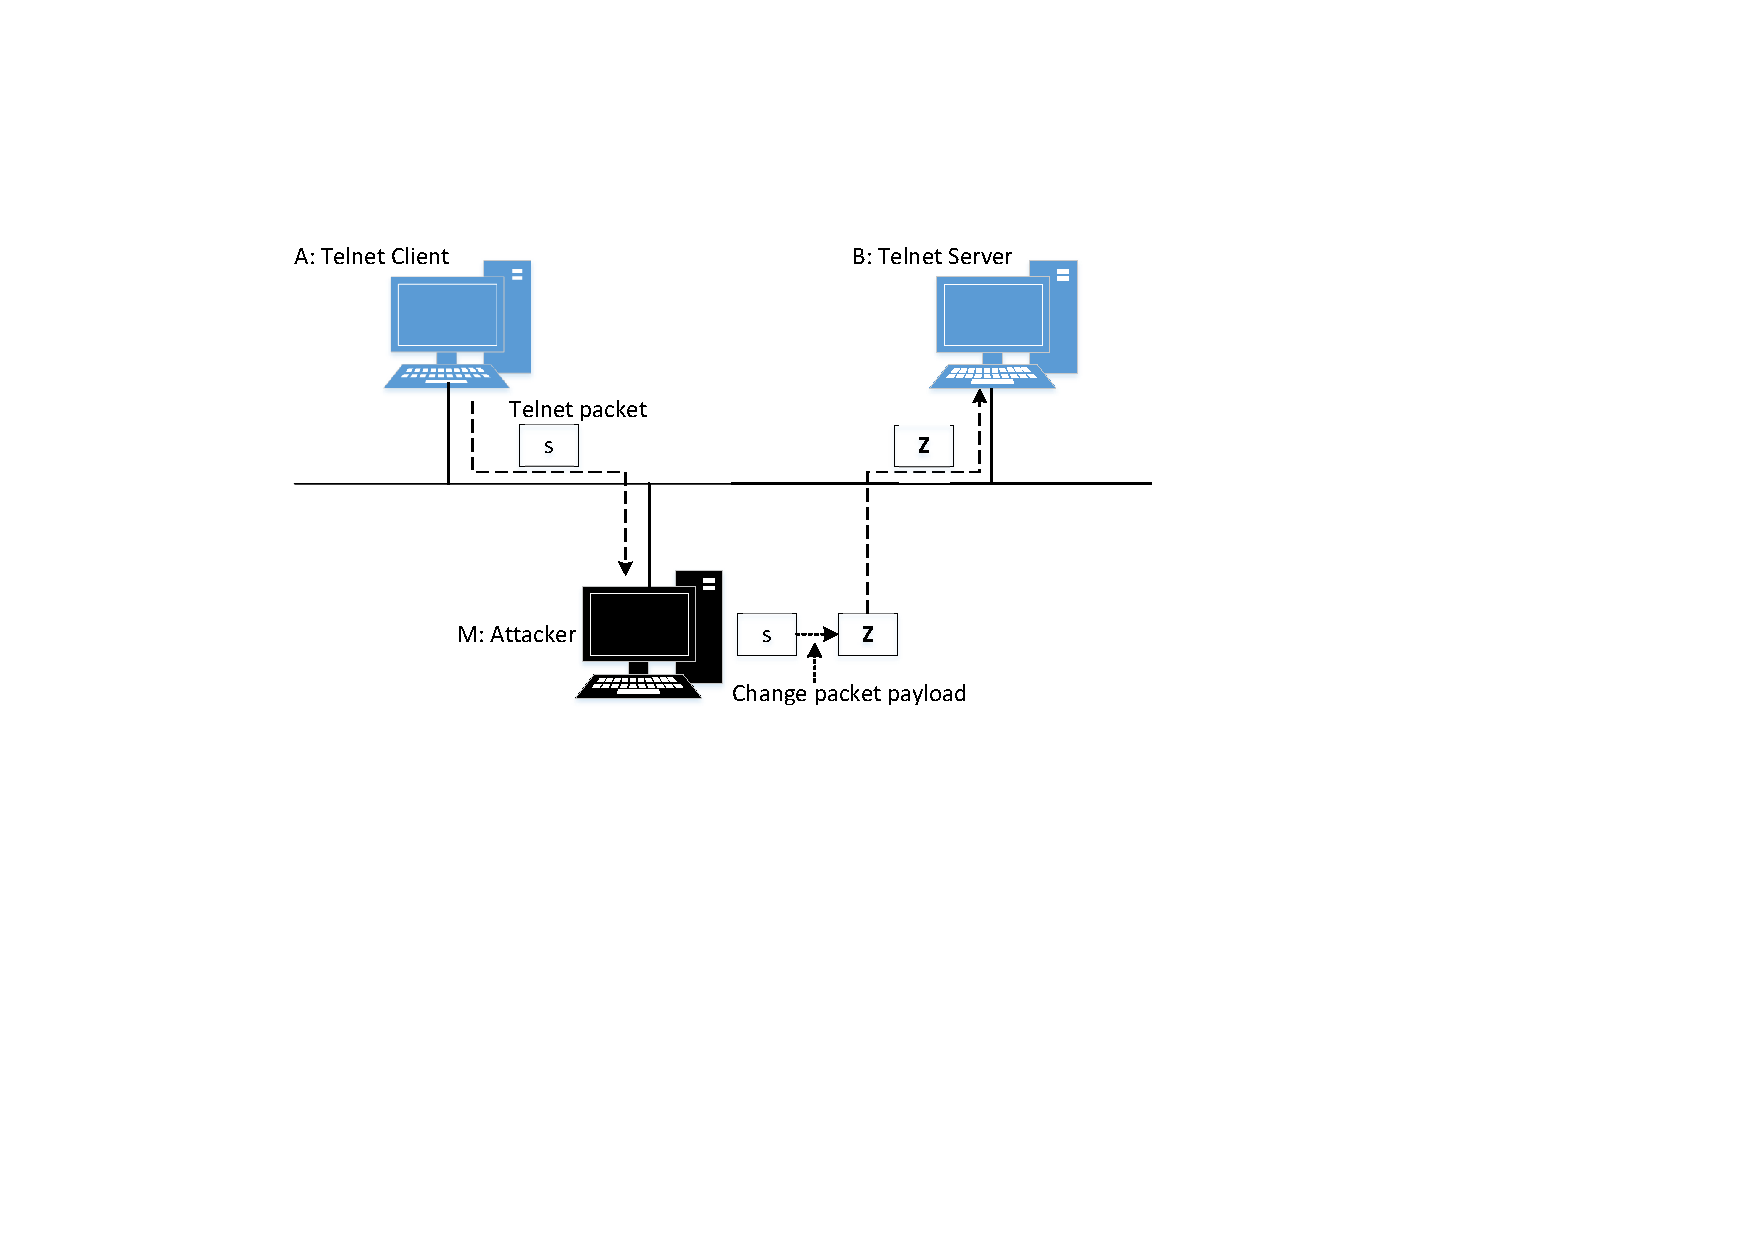
\includegraphics[width=0.8\textwidth]{\arpFigs/telnet_mitm.pdf}
    \caption{Man-In-The-Middle Attack against telnet}
    \label{arp:fig:telnet_mitm}
\end{figure}


\paragraph{Step 1 (Launch the ARP cache poisoning attack).} First, Host M conducts an ARP cache
poisoning attack on both A and B, such that in A's ARP cache, B's IP address maps to M's MAC
address, and in B's ARP cache, A's IP address also maps to M's MAC address. After this step,
packets sent between A and B will all be sent to M. We will use the ARP cache poisoning attack
from Task 1 to achieve this goal. It is better that you send out the spoofed packets
constantly (e.g. every 5 seconds); otherwise, the fake entries may be replaced by 
the real ones. 



\paragraph{Step 2 (Testing).} After the attack is successful, please try to ping each other
between Hosts A and B, and report your observation. Please show Wireshark results in your
report. Before doing this step, please make sure that the IP forwarding on Host M is turned
off. You can do that with the following command:

\begin{lstlisting}
# sysctl net.ipv4.ip_forward=0
\end{lstlisting}

\paragraph{Step 3 (Turn on IP forwarding).} Now we turn on the IP forwarding on Host M, so it
will forward the packets between A and B. Please run the following command and repeat Step 2.
Please describe your observation. 

\begin{lstlisting}
# sysctl net.ipv4.ip_forward=1
\end{lstlisting}

\paragraph{Step 4 (Launch the MITM attack).} We are ready to make changes to the Telnet data
between A and B. Assume that A is the Telnet client and B is the Telnet server. After A has
connected to the Telnet server on B, for every key stroke typed in A's Telnet window, a TCP
packet is generated and sent to B. We would like to intercept the TCP packet, and replace each
typed character with a fixed character (say Z). This way, it does not matter what the user
types on A, Telnet will always display Z.

From the previous steps, we are able to redirect the TCP packets to Host M, but instead of
forwarding them, we would like to replace them with a spoofed packet. We will write a
sniff-and-spoof program to accomplish this goal. In particular, we would like to do the
following: 

\begin{itemize}

\item We first keep the IP forwarding on, so we can successfully create a Telnet connection
between A to B. Once the connection is established, we turn off the IP forwarding using the
following command. Please type something on A's Telnet window, and report your observation: 

\begin{lstlisting}
# sysctl net.ipv4.ip_forward=0
\end{lstlisting}

\item We run our sniff-and-spoof program on Host M, such that for the captured packets sent
from A to B,  we spoof a packet but with TCP different data. For packets from B to A (Telnet
response), we do not make any change, so the spoofed packet is exactly the same as the original
one. 
\end{itemize} 

To help students get started, we provide a skeleton sniff-and-spoof
program below. The program captures all the TCP packets, and
then for packets from A to B, it makes some changes (the modification
part is not included, because that is part of the task). For packets from
B to A, the program does not make any change.  

\begin{lstlisting}
#!/usr/bin/env python3
from scapy.all import *

IP_A = "10.9.0.5"
MAC_A = "02:42:0a:09:00:05"
IP_B = "10.9.0.6"
MAC_B = "02:42:0a:09:00:06"


def spoof_pkt(pkt):
    if pkt[IP].src == IP_A and pkt[IP].dst == IP_B:
         # Create a new packet based on the captured one.
         # 1) We need to delete the checksum in the IP & TCP headers, 
         #    because our modification will make them invalid.
         #    Scapy will recalculate them if these fields are missing. 
         # 2) We also delete the original TCP payload.

         newpkt = IP(bytes(pkt[IP]))
         del(newpkt.chksum)
         del(newpkt[TCP].payload)
         del(newpkt[TCP].chksum)

         #################################################################
         # Construct the new payload based on the old payload.
         # Students need to implement this part.

         if pkt[TCP].payload:
             data = pkt[TCP].payload.load  # The original payload data
             newdata = data   # No change is made in this sample code

             send(newpkt/newdata)
         else:
             send(newpkt)
         ################################################################

    elif pkt[IP].src == IP_B and pkt[IP].dst == IP_A:
         # Create new packet based on the captured one 
         # Do not make any change 

         newpkt = IP(bytes(pkt[IP]))
         del(newpkt.chksum)
         del(newpkt[TCP].chksum)
         send(newpkt)


f = 'tcp'
pkt = sniff(iface='eth0', filter=f, prn=spoof_pkt)
\end{lstlisting}


It should be noted that the code above captures all the TCP 
packets, including the one generated by the program itself. That is 
undesirable, as it will affect
the performance. Students need to change the filter, so it does not capture
its own packets. 


\paragraph{Behavior of Telnet.}
In Telnet, typically, every character we type in the Telnet window triggers
an individual TCP packet, but if you type very fast, some characters may be 
sent together in the same packet. 
That is why in a typical Telnet packet from client to server, 
the payload only contains one character.  The
character sent to the server will be echoed back by the server, 
and the client will then display the
character in its window. Therefore, what we see in the client window is not the direct result
of the typing; whatever we type in the client window takes a round trip before it is displayed.
If the network is disconnected, whatever we typed on the client window will not displayed,
until the network is recovered. Similarly, if attackers change the character to Z during the
round trip, Z will be displayed at the Telnet client window, even though
that is not what you have typed.




% *******************************************
% SECTION
% ******************************************* 
\section{Task 3: MITM Attack on Netcat using ARP Cache Poisoning}

This task is similar to Task 2, except that
Hosts A and B are communicating using \texttt{netcat}, instead of \texttt{telnet}.
Host M wants to intercept their
communication, so it can make changes to the data sent between A and B.
You can use the following commands to establish a \texttt{netcat} TCP
connection between A and B:


\begin{lstlisting}
On Host B (server, IP address is 10.9.0.6), run the following:
# nc -lp 9090

On Host A (client), run the following:
# nc 10.9.0.6 9090
\end{lstlisting}
 

Once the connection is made, you can type messages on A.
Each line of messages will be put into a TCP packet sent 
to B, which simply displays the message.  
Your task is to replace every occurrence of your first name in the 
message with a sequence of A's. The length of the sequence should be the 
same as that of your first name, or you will mess up the TCP sequence
number, and hence the entire TCP connection. You need to use your real
first name, so we know the work is done by you.  



% *******************************************
% SECTION
% ******************************************* 
\section{Submission}


%%%%%%%%%%%%%%%%%%%%%%%%%%%%%%%%%%%%%%%%

You need to submit a detailed lab report, with screenshots,
to describe what you have done and what you have observed.
You also need to provide explanation
to the observations that are interesting or surprising.
Please also list the important code snippets followed by
explanation. Simply attaching code without any explanation will not
receive credits.

%%%%%%%%%%%%%%%%%%%%%%%%%%%%%%%%%%%%%%%%


\end{document}



